\section{Auswertung}
\label{sec:auswertung}

\section{Fehlerrechnung}
\label{subsec:fehlerrechnung}

\subsubsection{Mittelwert}
\begin{equation}
\overline{v} = \frac{1}{N} \sum_{i=1}^N v_i
\end{equation}

\subsubsection{Standardabweichung}
\begin{equation}
s_i = \sqrt{\frac{1}{N - 1} \sum_{j=1}^N \left(v_j - \overline{v}\right){^2}}
\end{equation}

wobei $v_j$ ($j = 1, ..., N$) die Messwerte sind.

\subsubsection{Streuung der Mittelwerte}
\begin{equation}
\sigma_i = \frac{s_i}{\sqrt{N}} = \sqrt{\frac{\sum_{j=1}^N \left(v_j - \overline{v_i}\right){^2}}{N \left(N - 1 \right)}}
\end{equation}

\subsubsection{Gaußfehler}
Bei einer fehlerbehafteten Funktion $f$ mit $k$ als fehlerbehafteter Größe und $\sigma_k$ als Ungenauigkeit, gilt:

\begin{equation}
\Delta x_k = \frac{\mathrm{d}f}{\mathrm{d}k}\sigma_k
\end{equation}.

 Der relative Gaußfehler berechnet sich nach:
\begin{equation}
\Delta x_\text{k, rel} = 1 \pm \frac{\Delta x_k}{|x|}\cdot 100\%
\end{equation}.

Der absolute Gaußfehler ergibt sich aus:
\begin{equation}
\Delta x_i = \sqrt{\left(\frac{\mathrm{d}f}{\mathrm{d}k_{1}}\cdot \sigma_{k_{1}}\right)^2 + \left(\frac{\mathrm{d}f}{\mathrm{d}k_{2}}\cdot \sigma_{k_{2}}\right)^2 + ...}
\end{equation}.


\subsection{Güteziffer}
  \label{subsec:güteziffer}
  Es soll die reale Güteziffer der Wärmepumpe ermittelt werden. Diese ergibt sich nach (\ref{eqn:güteziffer1}) und (\ref{eqn:güteziffer2}) zu
  \begin{equation}
    ν = \frac{(m_{1} c_w + m_k c_k)}{N}\frac {\mathrm{d}T_{1}}{\mathrm{d}t}.
  \end{equation}
  Der dort auftretende Differentialquotient $\frac {\mathrm{d}T_{1}}{\mathrm{d}t}$ lässt sich durch einen Fit der Messdaten an eine Funktion der Form
  \begin{equation}
    T(t) = \frac{A t^\alpha}{1+Bt^\alpha} + C
  \end{equation}
  errechnen. Die Messdaten ergeben die in Tabelle \ref{tab:koeffizienten} angegebenen Koeffizienten (von Einheiten wurde mangels physikalischen Sinns abgesehen):

  \begin{table}[!h]
    \centering
    \caption{Koeffizienten des nichtlinearen Fits.}
    \label{tab:koeffizienten}
    \sisetup{
      round-mode=places,
      round-precision=1,
    }
    \begin{tabular}{
        l@{}
        S[table-format=1.1e2] @{${}\pm{}$} S[table-format=1.1e2]
        S[table-format=1.1e2] @{${}\pm{}$} S[table-format=1.1e2]
        S[table-format=1.1e1] @{${}\pm{}$} S[table-format=1.1e2]
        S[table-format=1.1e0] @{${}\pm{}$} S[table-format=1.1e2]}
      \toprule
      & \multicolumn{2}{c}{$A$}
      & \multicolumn{2}{c}{$B$}
      & \multicolumn{2}{c}{$C$}
      & \multicolumn{2}{c}{$\alpha$} \\
      \midrule
      \input{coefficients.tex}
      \bottomrule
    \end{tabular}
  \end{table}
  Mithilfe der zeitlichen Ableitung von $T(t)$

  \begin{equation}
    \frac{\mathrm{d}T(t)}{\mathrm{d}t} = \frac{αAt^{α - 1} \cdot (1 + B t^α) - A t^α \cdot αBt^{α - 1}}{(1 + B t^ α)^ 2}
  \end{equation}

  und der Wärmekapazität $c_w = \SI{4.2 +- 0.04}{\kilo\joule\per\kilogram\per\kelvin}$ \cite[Dba2]{wärmeatlas} sowie Dichte von Wasser $\rho = \SI{994(10)}{\kilogram\per\meter\cubed}$ \cite[Dba2]{wärmeatlas} und der angegebenen Wärmekapazität der Apparatur $c_km_k = \SI{750(10)}{\joule\per\kelvin}$ kann dann die Güteziffer zu verschiedenen Zeitpunkten ermittelt werden.

  Im Vergleich dazu sollte nach (\ref{eqn:güte_ideal}) zu den selben Zeitpunkten die Güteziffer einer idealen Wärmepumpe ermittelt werden, die bei den entsprechenden Temperaturniveaus arbeitet.
  Die Ergebnisse sind Tabelle \ref{tab:ergebnisse_güte} und Abb. \ref{fig:temperatur} zu entnehmen.

  \begin{table}[h]
    \centering
    \caption{Ermittelte Gütezahlen.}
    \label{tab:ergebnisse_güte}
    \sisetup{
      round-mode=places,
      round-precision=3,
    }
    \begin{tabular}{
        l@{}
        S[table-format=4.0]
        S[table-format=1.3] @{${}\pm{}$} S[table-format=1.3]
        S[table-format=2.3] @{${}\pm{}$} S[table-format=1.3]
        S[table-format=2.3] @{${}\pm{}$} S[table-format=1.3]}
      \toprule
      & $t / \si{\second}$
      & \multicolumn{2}{c}{$ν$}
      & \multicolumn{2}{c}{$ν_{\mathrm{ideal}}$}
      & \multicolumn{2}{c}{$ν / ν_{\mathrm{ideal}}$} \\
      %& \multicolumn{2}{c}{$\dot m / \si{\gram\per\second}$}
      %& \multicolumn{2}{c}{$N / \si{\watt}$} \\
      \midrule
      \input{table_guete.tex}
      \bottomrule
    \end{tabular}
  \end{table}

  \begin{figure}[htpb]
    \centering
    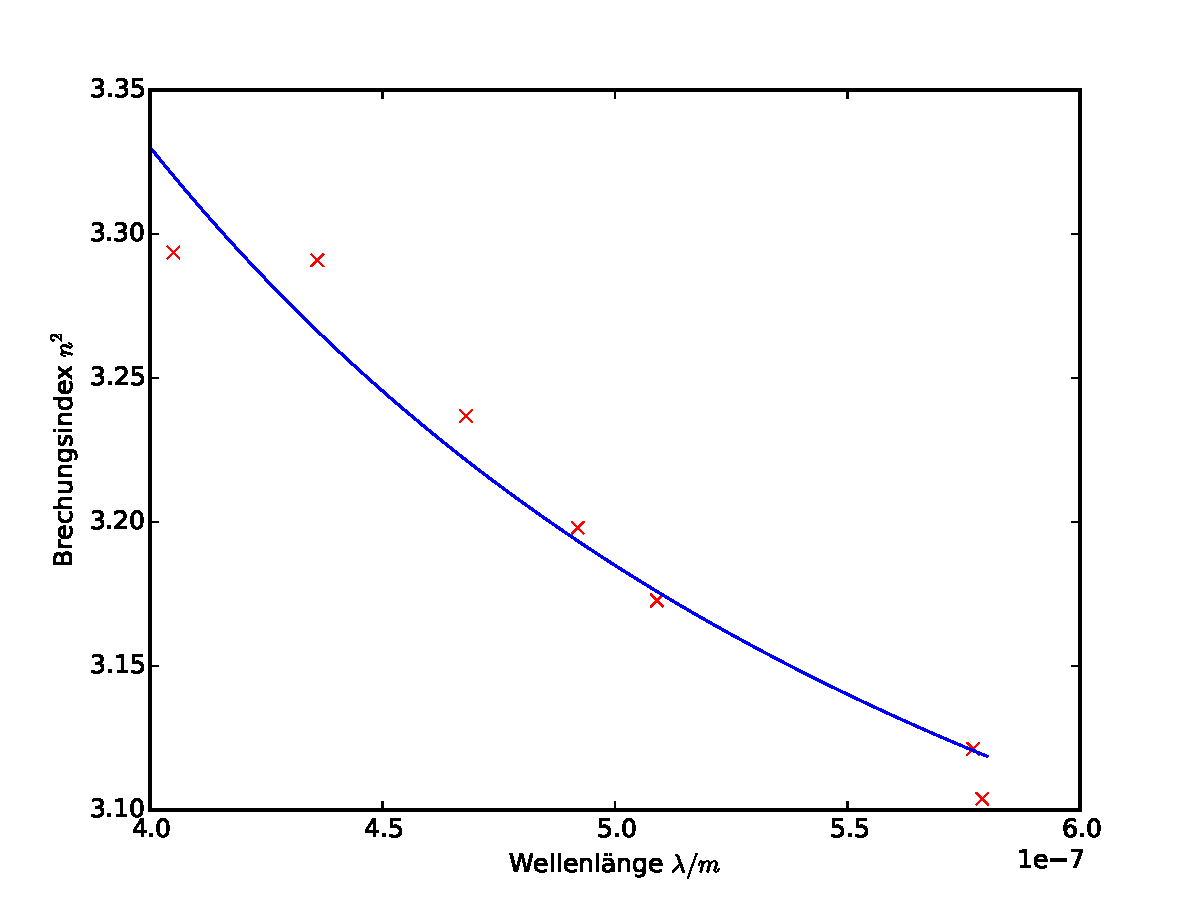
\includegraphics{plot.pdf}
    \caption{Plot des Temperaturverlaufs und der Fits.}
    \label{fig:temperatur}
  \end{figure}

\newpage
\subsection{Massendurchsatz}
  Außerdem soll der Massendurchsatz des Kreislaufes ermittelt werden. Dies geschieht, indem (\ref{eqn:durchsatz1}) und (\ref{eqn:durchsatz2}) zu
  \begin{equation}
    \frac{\mathrm{d}m}{\mathrm{d}t} = \dot m = \frac{(m_{2} c_w + m_k c_k)}{L}\frac {\mathrm{d}T_{2}}{\mathrm{d}t}
  \end{equation}
  umgestellt werden. Der Differentialquotient $\frac {\mathrm{d}T_{2}}{\mathrm{d}t}$ wird exakt wie in Abschnitt \ref{subsec:güteziffer} mittels nichtlinearer Ausgleichsrechnung bestimmt. Die Verdampfungswärme $L$ lässt sich aus der (vom Manometer abgelesenen) Dampfdruckkurve von Dichlordifluormethan (Tabelle \ref{tab:dampfdruck}) mithilfe einer linearen Regression des logarithmierten Drucks über die reziproke Temperatur ermitteln. Es gilt nach \cite{anleitung203}
  \begin{equation}
    \ln p = -\frac{L}{R} \frac {1}{T} + \mathrm{const.}
  \end{equation}
  Damit ergibt sich $L$ zu $-R \cdot a$ mit der Steigung $a$ der Ausgleichsgeraden und der universellen Gaskonstante $R = \SI[separate-uncertainty=false]{8.3144598(48)}{\joule\per\mol\per\kelvin}$\cite{codata}. Der Durchsatz in \si{\mol\per\second} wird noch mit der molaren Masse $M = \SI{120.913}{\gram\per\mol}$\cite[267]{gase} des Kältemittels multipliziert um nicht nur die Anzahl der Moleküle, sondern die Masse zu erhalten. Eine grafische Darstellung der Dampfdruckkurve findet sich in Abb. \ref {fig:dampfdruck}, die Ergebnisse für den Massendurchsatz in Tabelle \ref{tab:ergebnisse_durchsatz}, wobei das negative Vorzeichen, welches die \enquote{Flussrichtung} der Masse bestimmt, ignoriert wird.

  \begin{table}[htbp]
    \centering
    \caption{Ermittelte Massendurchsätze.}
    \label{tab:ergebnisse_durchsatz}
    \sisetup{
      round-mode=places,
      round-precision=3,
    }
    \begin{tabular}{
        l@{}
        S[table-format=4.0]
        S[table-format=1.3] @{${}\pm{}$} S[table-format=1.3]}
      \toprule
      & $t / \si{\second}$
      & \multicolumn{2}{c}{$\dot m / \si{\gram\per\second}$} \\
      \midrule
      \input{table_massendurchsatz.tex}
      \bottomrule
    \end{tabular}
  \end{table}

  \begin{figure}[htpb]
    \centering
    \includegraphics{plot_dampfdruck.pdf}
    \caption{Plot der Dampfdruckkurve.}
    \label{fig:dampfdruck}
  \end{figure}

  \begin{table}[htbp]
    \centering
    \caption{Dampfdruckkurve von Dichlordifluormethan.}
    \label{tab:dampfdruck}
    \begin{tabular}{l@{}
        S[table-format=3.2]
        S[table-format=4.0]
      }
      \toprule
      & $T / \si{\kelvin}$
      & $p/ \si{\kilo\pascal}$\\
      \midrule
      \input{table_dampfdruck.tex}
      \bottomrule
    \end{tabular}
  \end{table}

\subsection{Mechanische Kompressorleistung}
  Zuletzt sollte die menchanische Leistung des Kompressors ermittelt werden. Diese ist nach (\ref{eqn:mechleistung})
  \begin{equation}
    N_\mathrm{mech} = \frac{1}{\kappa-1}\biggl(p_b \sqrt[\kappa]{\frac{p_a}{p_b}}-p_a\biggr)\frac{1}{\rho} \frac{\mathrm{d}m} {\mathrm{d}t}.
  \end{equation}
  Dabei ist die Dichte $\rho$ mithilfe der allgemeinen Gasgleichung zu bestimmen:

  \begin{align}
    pV &=nRT \\
    \Leftrightarrow \frac{pV}{T} &= nR
    \intertext{Im geschlossenen System gilt: $nR = \mathrm{const.}$ Also ist }
    \frac{p_0 V_0}{T_0} &= \frac{p_2 V_2}{T_2}
    \intertext{mit $V = \frac{m}{\rho}$ folgt}
    \frac{p_0 m_0}{\rho_0 T_0} &= \frac{p_2 m_2}{\rho_2 T_2},
    \intertext{da $m_0 = m_2$ ergibt sich}
    \frac{p_0}{\rho_0 T_0} = \frac{p_2}{T_2 \rho_2} &\Leftrightarrow \rho_2 = \frac{\rho_0 T_0 p_2}{T_2 p_0}
    \intertext{mit $\rho_{2} = \rho$ und $p_{2} = p_a$ also}
    \rho &= \frac {\rho_0 T_0 p_a}{T_2 p_0}
  \end{align}

  In der Versuchsanleitung\cite{anleitung206} sind die Werte $\rho_{0} = \SI{5.51}{\gram\per\liter}$, $p_{0} = \SI{1}{\bar}$, $T_{0} = \SI{0}{\celsius}$ und $\kappa = \num{1.14}$ gegeben, die restlichen Größen werden den Messdaten entnommen. Die berechneten mechanischen Kompressorleistungen finden sich in Tabelle \ref{tab:ergebnisse_leistung}.

  \begin{table}[htpb]
    \centering
    \caption{Ermittelte Leistungen.}
    \label{tab:ergebnisse_leistung}
    \sisetup{
      round-mode=places,
      round-precision=3,
    }
    \begin{tabular}{
        l@{}
        S[table-format=4.0]
        S[table-format=2.3] @{${}\pm{}$} S[table-format=2.3]}
      \toprule
      & $t / \si{\second}$
      & \multicolumn{2}{c}{$N / \si{\watt}$} \\
      \midrule
      \input{table_kompressorleistung.tex}
      \bottomrule
    \end{tabular}
  \end{table}
  \newpage

  \newgeometry{top=3cm, bottom=5cm}
  \subsection{Messdaten}
  \begin{table}[htpb]
    \tiny
    \centering
    \caption{Messdaten.}
    \label{tab:messdaten}
    \begin{tabular}{l@{}
        S[table-format=4.0]
        S[table-format=3.2]
        S[table-format=3.2]
        S[table-format=3.0]
        S[table-format=4.0]
        S[table-format=3.0]
      }
      \toprule
      & $t / \si{\second}$
      & $T_{1} / \si{\kelvin}$
      & $T_{2} / \si{\kelvin}$
      & $p_a / \si{\kilo\pascal}$
      & $p_b / \si{\kilo\pascal}$
      & $P / \si{\watt}$ \\
      \midrule
      \input{table_data.tex}
      \midrule
      \multicolumn{7}{c}{Messunsicherheiten:}\\
      \multicolumn{7}{c}{$\Delta T = \SI{0.1}{\kelvin}, \Delta p_a = \SI{0.2}{\bar}, \Delta p_b = \SI{1}{\bar}, \Delta V = \SI{0.4}{\milli\liter}$}\\
      \bottomrule
    \end{tabular}
  \end{table}
  \restoregeometry
